\documentclass[10pt,aspectratio=43]{beamer}
\usepackage{bibentry}
\usepackage[style=bwl-FU]{biblatex}
\usepackage[dvipsnames]{xcolor}
\usepackage{graphicx} % Allows including images
\usepackage{booktabs} % Allows the use of \toprule, 
\usepackage{array}
\usepackage{wrapfig}
\usepackage{graphics}
\usepackage{graphicx}
\usepackage{amsfonts}
\usepackage{amssymb}
\usepackage{amsthm}
\usepackage{textcomp}
% \usepackage{enumitem}
\usepackage{graphicx} % Allows including images
\usepackage{booktabs} % Allows the use of \toprule, 
% \usepackage[nottoc]{tocbibind}
\usepackage{threeparttable}
% \usepackage{natbib}
% \usetheme{SimpleDarkBlue}

% \usepackage{mathrsfs}
\usepackage[nospace]{varioref}	
\usepackage{cleveref}

\usepackage{presentation}

\setlength{\parskip}{\baselineskip} 
% \graphicspath{{./../Figures}}
% \setlength\itemsep{2em}

\setlength\belowcaptionskip{-3ex}


\usepackage{caption}
\usepackage{subcaption}

\bibliography{references.bib}


\usepackage{makecell}

% \usecolortheme{}
\usepackage{amsmath}


\DeclareMathOperator*{\argmax}{arg\,max}
\DeclareMathOperator*{\argmin}{arg\,min}


\title{Bayesian Estimation of Risk-Neutral Probability}
% Enter presentation information:
\information%
% Enter link to research paper (optional; comment line if not needed):
%[]%
% Enter presentation authors:
{Alexander Vlasov (avlasov@nes.ru)}%
% Enter presentation location and date (optional; comment line if not needed):
{New Economic School -- 2025-06-20}

% \usecolortheme{}

% \AtBeginSection{
% 	\begin{frame}[fragile]\Large	
% 		\frametitle{Contents}
% 		\tableofcontents[currentsection]
% 	\end{frame}
% }
% \setbeamerfont{footnote}{size=\tiny}


% \setbeamerfont{normal text}{size=\small}
% \AtBeginDocument{\usebeamerfont{normal text}}


\graphicspath{{../Figures/}}

\begin{document}

\begin{frame}[fragile]
    \titlepage
\end{frame}



% \section{Limitations of RA models}
% \begin{frame}[fragile]{Contents}
%     \large
%     \tableofcontents[currentsection]
% \end{frame}

\begin{frame}{\al{Implied} Risk-Neutral Probability Density}

    \[S=\sum_{s=1}^K\phi(s)q(s)\]

    \[\phi^*\overset{d}{=}\frac{\phi(s)}{\sum_{s=1}^K\phi(s)}=\frac{\phi(s)}{1/(1+r)}=(1+r)\phi(s)\]

    \[S=\frac{1}{1+r}\sum_{s=1}^K\phi^*(s)q(s)=\frac{1}{1+r}\mathbb{E}^*[q(s)].\]

\end{frame}
\begin{frame}{Implied \al{Risk-Neutral} Probability Density}
 
    For TAS utility, the state-prices are 
    \[\phi(s)=\pi\frac{\beta u'[c(s)]}{u'[c(0)]},\]
    \then implied risk-neutral probability is
    \[\phi^*(s)=\pi\frac{\beta u'[c(s)]}{u'[c(0)]}(1+r)= \pi\frac{u'[c(s)]}{u'[c(0)]}\approx \pi,\]
    for $u'$ is constant (risk-neutrality) or $c(s)\approx c(0)~\forall s$.


\end{frame}

\begin{frame}{Breeden-Litzenberger (1978) Formula}
\nocite{breedenPricesStateContingentClaims1978}
For short-term, $r\approx 0$.
    \begin{align*}
        C(S,t)&=\mathbb{E}^*\left[[S(T)-\mathcal{K}]^+\mid S(t)=S\right]\\ 
        &=\int_0^{+\infty}(x-\mathcal{K})^+\,dP^*(x)\\ &=\int_{\mathcal{K}}^{+\infty}x\,dP^*(x)-\mathcal{K}\int_0^{+\infty}\,dP^*(x)\\ 
        &=\int_{\mathcal{K}}^{+\infty}x\,dP^*(x)-\mathcal{K}(1-P^*(\mathcal{K}))
    \end{align*}
    \begin{align*}
        \frac{\partial C}{\partial \mathcal{K}}&=-\mathcal{K}p^*(\mathcal{K})-1+P^*(\mathcal{K})+\mathcal{K}p^*(\mathcal{K})=P^*(\mathcal{K})-1\\ 
        \frac{\partial^2 C}{\partial \mathcal{K}^2}&=p^*(\mathcal{K}).
    \end{align*}
 \cite{ait-sahaliaNonparametricOptionPricing2003}

\end{frame}



\begin{frame}{Bayesian Formulation}
    \cite{fisherSimplexRegression2016} proposes the following approach.

    \[y_i=\lambda\sum_{j=1}^KX_{ij}\beta_j+\varepsilon_i,\]
    where $\beta=(\beta_1,\dots, \beta_K)\in \Delta^{K-1}$, $\Delta^{K-1}$ denotes the simplex of dimension $(K-1)$; $X_{ij}$ is a payoff of derivative $i$ in state $j$, and $\varepsilon_i\sim N(0,\sigma^2)$.

    In vector form,
    \[y=\lambda X \beta+\varepsilon.\]

    In order to insure $\beta\in \Delta^{K-1}$, we select the (symmetric) Dirichlet prior:
    \[p(\beta\mid \alpha)=\operatorname{Dirichlet}(\beta\mid \alpha)\propto \prod_{i=1}^{K}x_{i}^{\alpha-1}.\]

\end{frame}

\begin{frame}{}
$X$ consists of $n$ payoffs of $K$ derivatives, including the payoffs price (you can think of it as call option with strike equal zero).

The state space is chosen to ensure that the first and last coefficients are near zero, so the list of possibilities is exhaustive.
 \begin{center}
        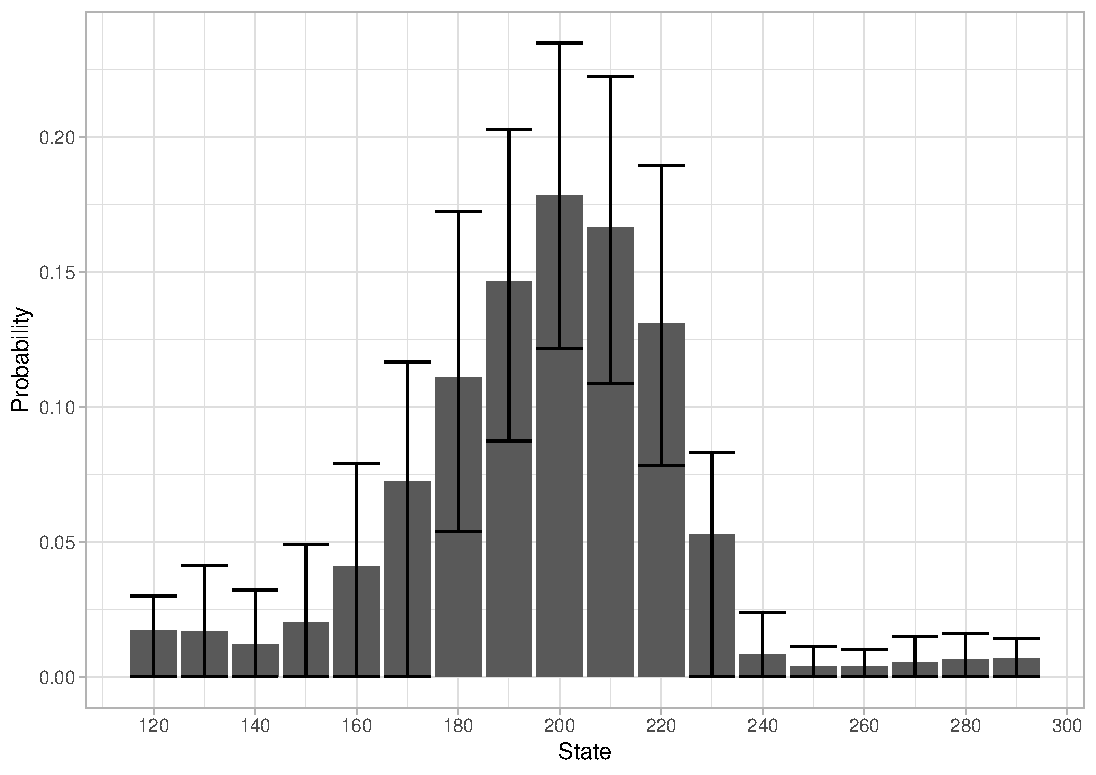
\includegraphics[width=0.6\linewidth]{betas_23_3.pdf}
    \end{center}

\end{frame}

\begin{frame}{Prior for Concentration Coefficient}
    $\alpha$ is a vector of concentration parameters for Dirichlet distribution. 
    
    It is reasonable to select a distribution that is relatively flat on $[0,1]$ and assign a large portion of mass to $[0,1]$. \cite{fisherSimplexRegression2016} uses Lognormal prior, I propose Weibull. The result turns out to be almost identical.

    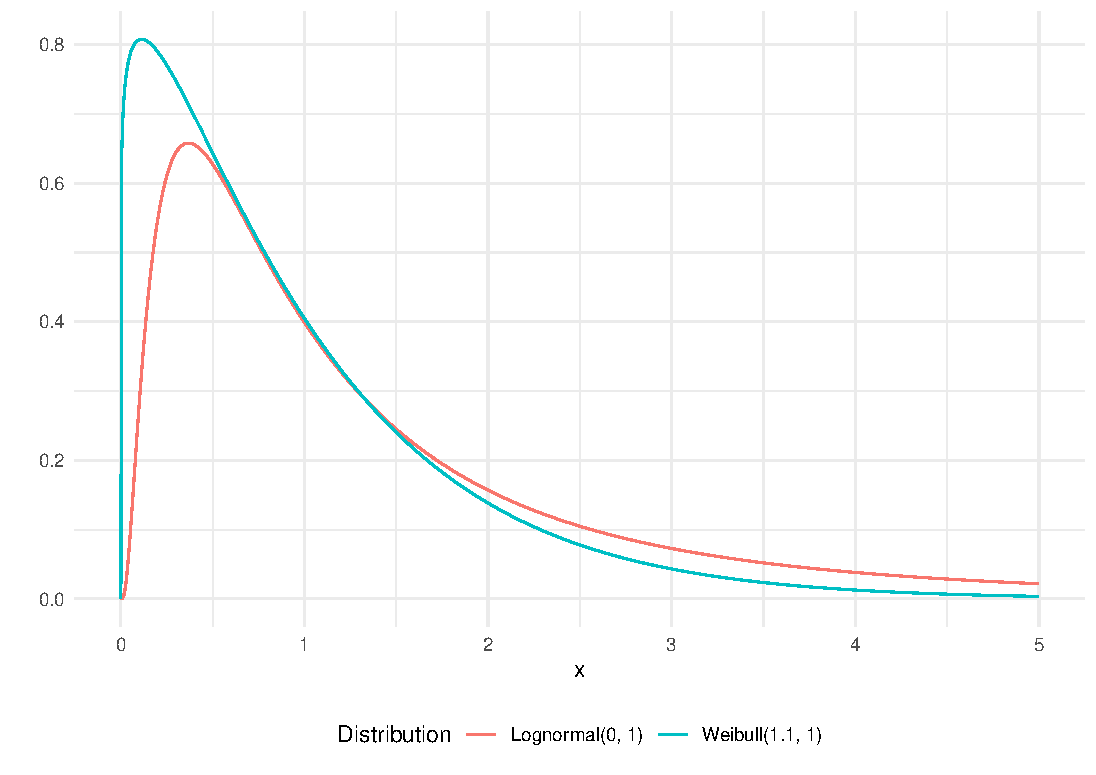
\includegraphics[width=0.6\textwidth]{prior_difference.pdf}

\end{frame}

\begin{frame}{Priors and Posterior}
     \[p(\beta\mid \alpha)=\operatorname{Dirichlet}(\beta\mid \alpha)\propto \prod_{i=1}^{K}x_{i}^{\alpha-1}.\]
    \[p(\alpha)=\operatorname{Weibull}(1.1,1)\]
    \[p(\sigma^2)\propto \frac{1}{\sigma^2}\]

    \[p(\alpha,\lambda,\sigma,\beta\mid y)\propto N(y\mid \lambda X\beta,\sigma)\times\operatorname{Dirichlet}(\beta\mid \alpha)\times \frac{1}{\sigma^2}\]

\end{frame}





\begin{frame}{Risk Neutral Density for AAPL I}
    Calculated in 2025-05-23 with expiration date 2025-06-13. Wiskers are 90\% HPD interval.
    \begin{center}
        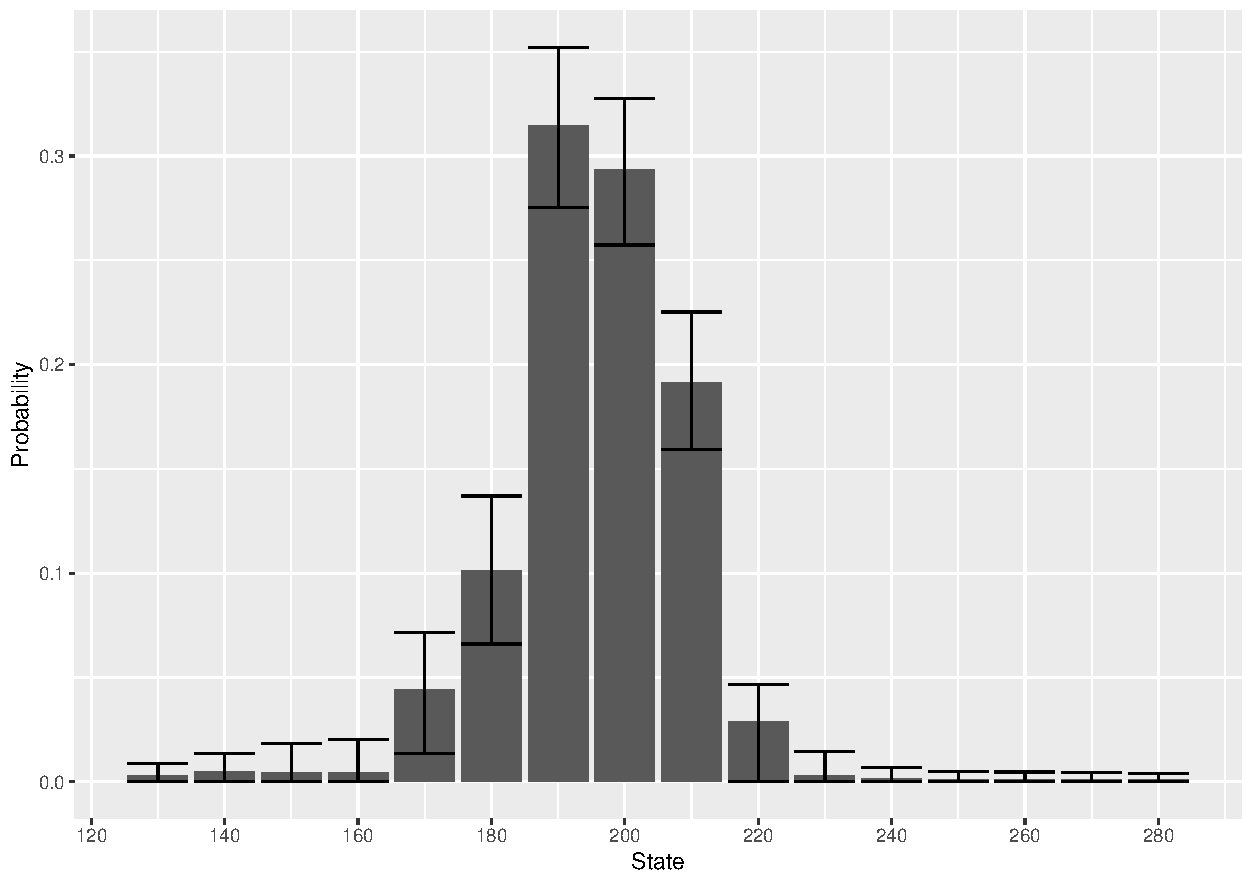
\includegraphics[width=0.8\linewidth]{betas_23_1.pdf}
    \end{center}
    
\end{frame}

\begin{frame}{Risk Neutral Density for AAPL II}
    Calculated in 2025-05-23 (same) with expiration date 2025-07-18 (\al{+35 days}).
    \begin{center}
        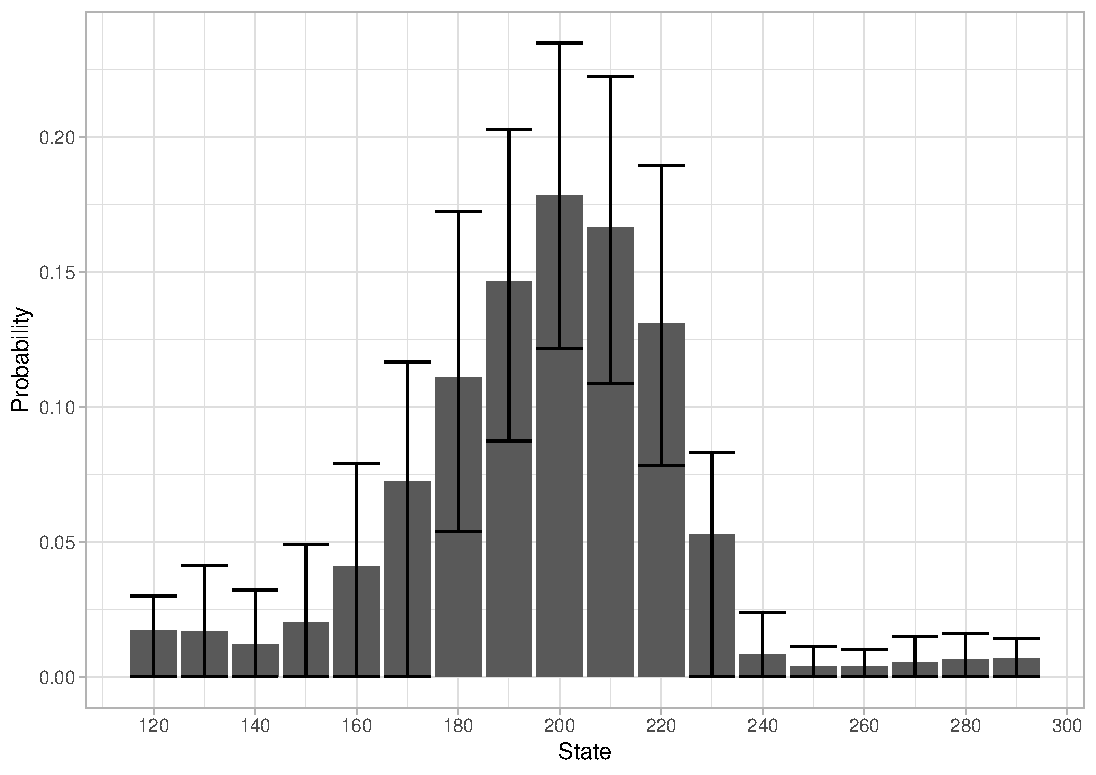
\includegraphics[width=0.8\linewidth]{betas_23_3.pdf}
    \end{center}
    
\end{frame}

\begin{frame}{Estimates of Implied Risk-Neutral Density}\centering
    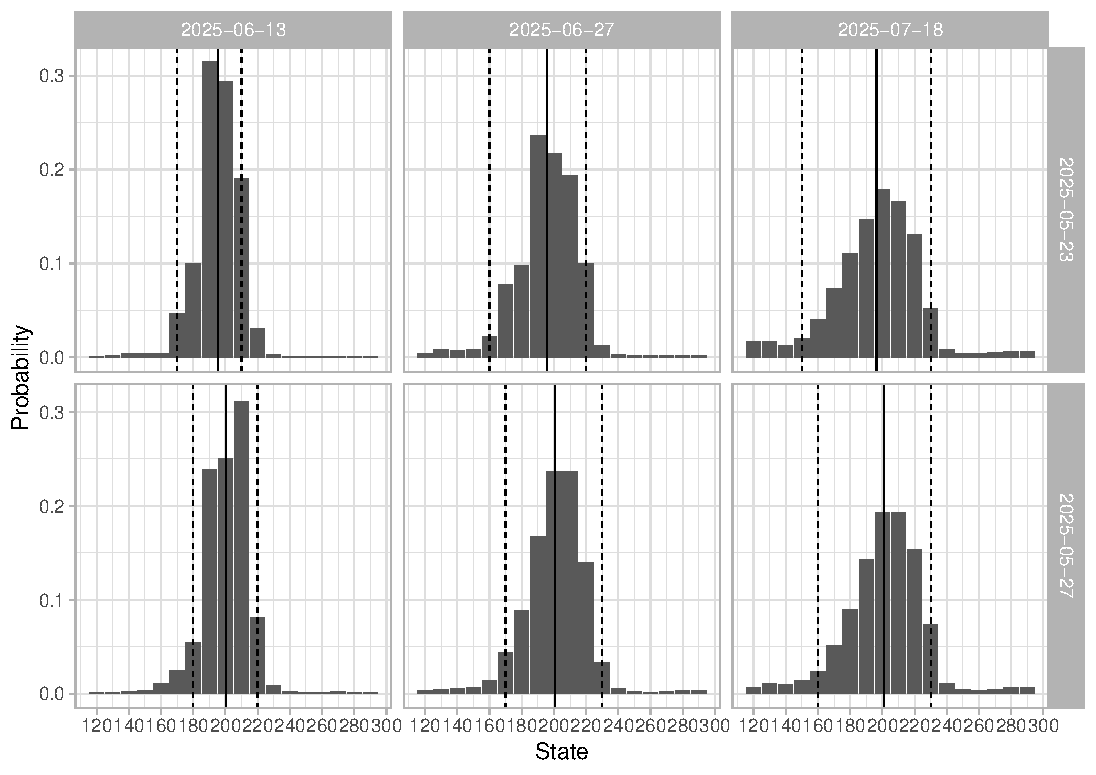
\includegraphics[width=\linewidth]{betas.pdf}
\end{frame}
 

\begin{frame}{Summary Statistics}
    \begin{center}
        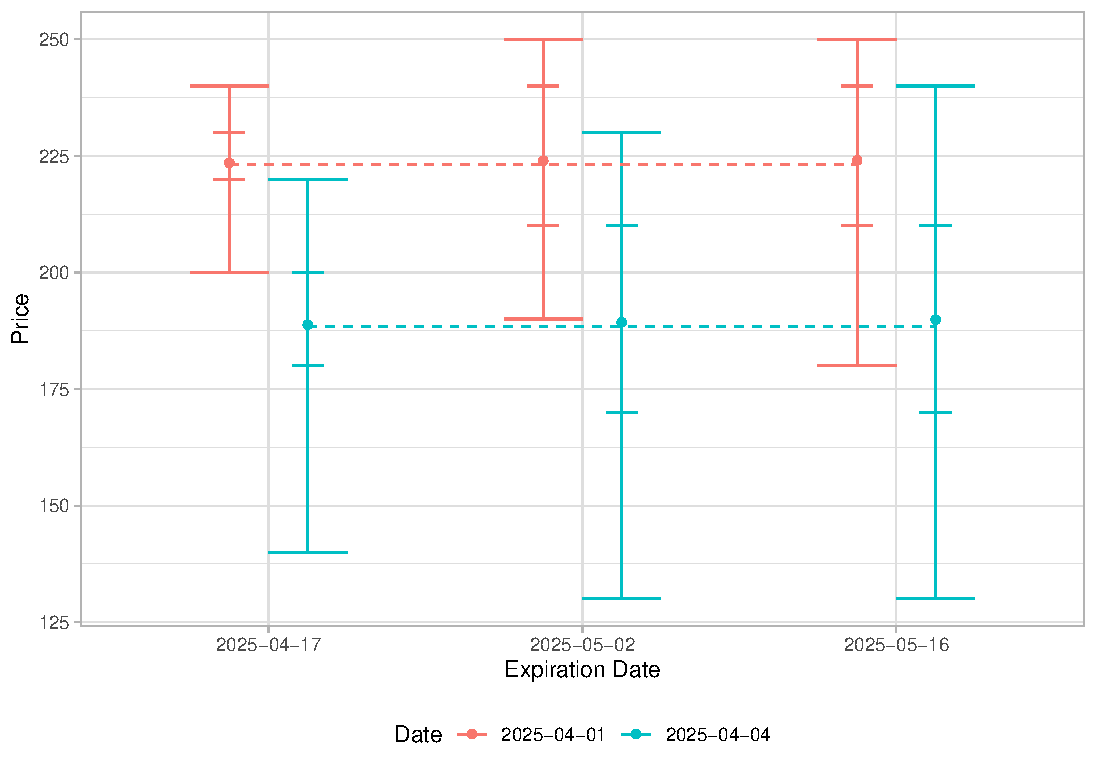
\includegraphics[width=0.9\linewidth]{summaries_plot.pdf}
    \end{center}
\end{frame}


\begin{frame}{Concentration Parameter Estimates}
    \centering
    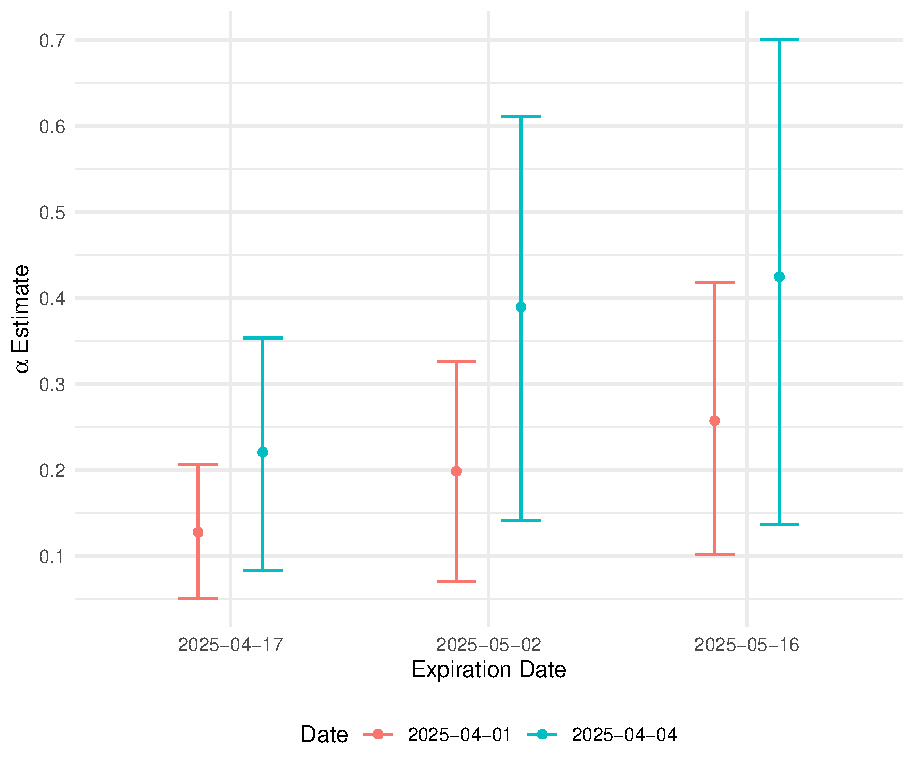
\includegraphics[scale=0.6]{alphas.pdf}
\end{frame}

% \begin{frame}{Alpha Distribution}
%     \centering
%     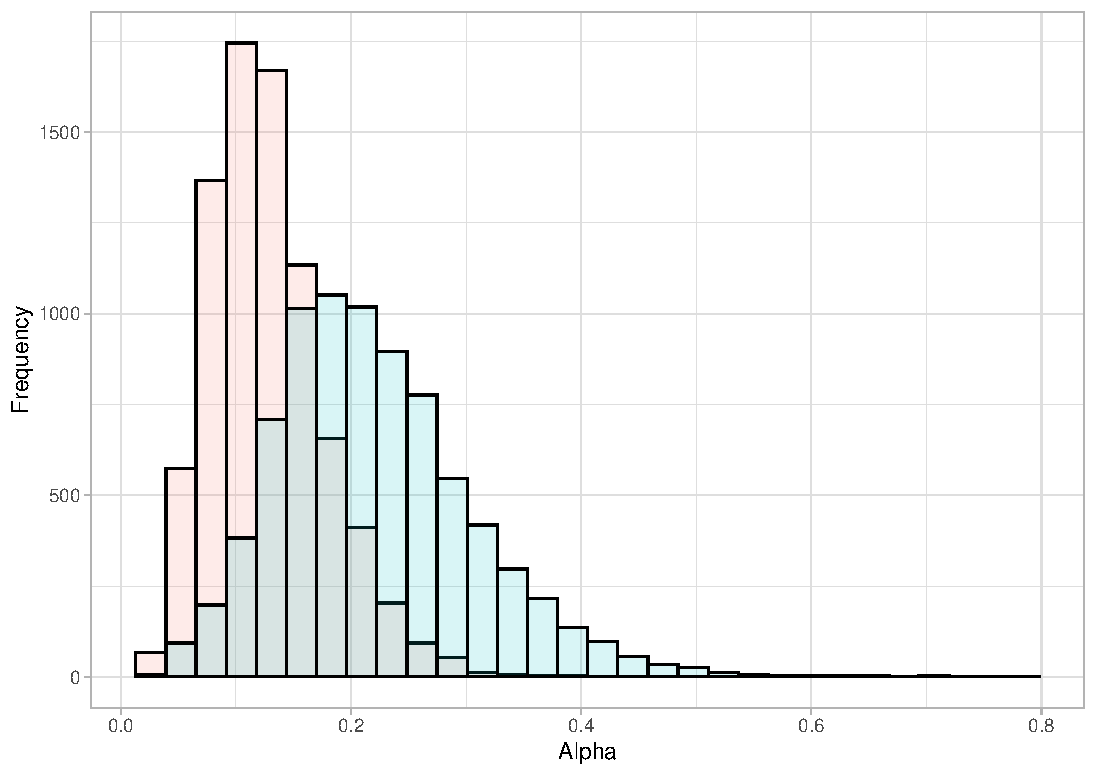
\includegraphics[width=0.8\linewidth]{alpha_histogram.pdf}
% \end{frame}

% \begin{frame}{Use Cases}
%     123
% \end{frame}


\lastslide

\begin{frame}[allowframebreaks]{References}
    \renewcommand*{\bibfont}{\scriptsize}
    \printbibliography
\end{frame}

% \appendix 

% \begin{frame}
    
% \end{frame}


\end{document}